%%% LaTeX Template: Article/Thesis/etc. with colored headings and special fonts
%%%
%%% Source: http://www.howtotex.com/
%%% Feel free to distribute this template, but please keep to referal to http://www.howtotex.com/ here.
%%% February 2011

%%%%% Preamble
\documentclass[10pt,a4paper]{article}

\usepackage[T1]{fontenc}
\usepackage[bitstream-charter]{mathdesign}

%\usepackage[latin1]{inputenc}							% Input encoding

\usepackage[turkish]{babel}
\usepackage[utf8]{inputenc} 
\usepackage{amsmath} 
\usepackage{gensymb}									%Derece sembolü için gerekli paket
\usepackage{subcaption}									%subfigure icin 

\usepackage{graphicx}
\graphicspath{ {images/} }	%resim dosyalari klasörü

\usepackage{xcolor}			%Caf cafli tablo icin gerekli
\definecolor{bl}{rgb}{0.0,0.2,0.6} 

%Caf cafli tablo icin
\usepackage{colortbl}
\usepackage{array}
\usepackage{booktabs}
\newcommand*{\arraycolor}[1]{\protect\leavevmode\color{#1}}
\newcolumntype{A}{>{\columncolor{blue!50!white}}c}
\newcolumntype{B}{>{\columncolor{LightGoldenrod}}c}
\newcolumntype{C}{>{\columncolor{FireBrick!50}}c}
\newcolumntype{D}{>{\columncolor{Gray!42}}c}
%

\usepackage{sectsty}
\usepackage[compact]{titlesec} 
\allsectionsfont{\color{bl}\scshape\selectfont}

%%%%% Definitions
% Define a new command that prints the title only
\makeatletter							% Begin definition
\def\printtitle{%						% Define command: \printtitle
	{\color{bl} \centering \huge \sc \textbf{\@title}\par}}		% Typesetting
\makeatother							% End definition

\title{Asenkron Motorların \\ 
	\large \vspace*{-10pt} Skaler ve Vektörel Kontrolü\vspace*{10pt}}

% Define a new command that prints the author(s) only
\makeatletter							% Begin definition
\def\printauthor{%					% Define command: \printauthor
	{\centering \small \@author}}				% Typesetting
\makeatother							% End definition

\author{%
	NAZIM YILDIZ \\
	nazimyildiz90@gmail.com \\
	\vspace{20pt}
}

% Custom headers and footers
\usepackage{fancyhdr}
\pagestyle{fancy}					% Enabling the custom headers/footers
\usepackage{lastpage}	
% Header (empty)
\lhead{}
\chead{}
\rhead{}
% Footer (you may change this to your own needs)
\lfoot{\footnotesize \texttt{www.pau.edu.tr/} - Rapor}
\cfoot{}
\rfoot{\footnotesize page \thepage\ of \pageref{LastPage}}	% "Page 1 of 2"
\renewcommand{\headrulewidth}{0.0pt}
\renewcommand{\footrulewidth}{0.4pt}

% Change the abstract environment
\usepackage[runin]{abstract}			% runin option for a run-in title
\setlength\absleftindent{30pt}		% left margin
\setlength\absrightindent{30pt}		% right margin
\abslabeldelim{\quad}						% 
\setlength{\abstitleskip}{-10pt}
\renewcommand{\abstractname}{}
\renewcommand{\abstracttextfont}{\color{bl} \small \slshape}	% slanted text


%%% Start of the document
\begin{document}
	%%% Top of the page: Author, Title and Abstact
	\printtitle 
	
	\printauthor
	
	\begin{abstract}
		Bu çalışmada asenkron motoların kontrolünde yaygın bir şekilde kullanılan skaler yani 
		$\frac{V}{f}$ ve vektörel kontrol yöntemleri tanıtılmış, arasındaki farklar incelenmistir.
		
			\begin{figure}[hp]
				\centering	
				\shorthandoff{=}
				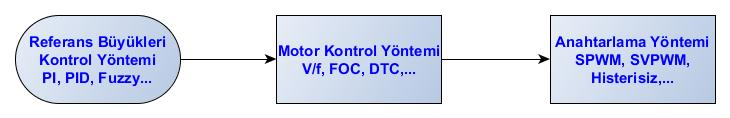
\includegraphics[width=1.0\linewidth]{MotorKontrolDiyagram.jpg}
				\shorthandon{=}	
				\caption{Motor Sürme Aşamaları}
				\label{fig:motordrive}
			\end{figure}
			
			Ayrıca genel olarak 3 yada çok fazlı motorları sürerken şekil-\ref{fig:motordrive} deki aşamalar uygulamaya göre değerlendirilerek ihtiyaç doğrultusunda aralarında seçim yapılır.
	\end{abstract}
	
	%%% Start of the 'real' content of the article, using a two column layout
	\section{Skaler Kontrol}
	$\frac{V}{f}$ kontrolü adıylada anılan basit ve matematiksel anlamda mikrodenetleyicileri yormayan sade bir yapısı vardır.
	Yöntemin çalışma felsefesi ise frekans arttıkça yani makine hızlandıkça voltaj da doğrulsal bir şekilde arttırılarak makina akısının sabit tutulmaya çalışıldığı bir tekniktir. Şekil-\ref{fig:vf_kar} de bu karakteristik verilmiştir. Matematiksel karşılığı ise $\frac{Vrms}{f} = 4.44 \times N \times {\Phi_s} \times C$ burada C nüve katsayısıdır.\newline

	\begin{figure}[hp]
		\centering	
		\shorthandoff{=}
		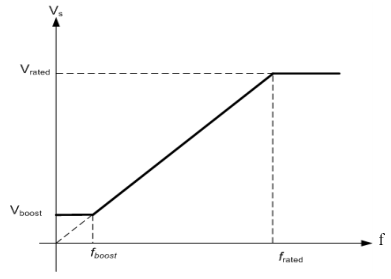
\includegraphics[width=0.7\linewidth]{vf_grafigi.png}
		\shorthandon{=}	
		\caption{V/f Akı Kontrol Karakteristiği}
		\label{fig:vf_kar}
	\end{figure}
	
	Şekil-\ref{fig:vf_kar} de görüldüğü üzere 3 bölge bulunmaktadır. Bu bölgeler $0-f_{boost}$ aralığı motorun yük altında kalkabilmesini sağlayan nominal akı limitlerinin üzerine çıkıldığı bölge ve motor bu bölgenin dışına çıktıktan sonra durmadığı sürece bu bölgedeki çalışma tekrar uygulanmaz, $f_{boost}-f_{rated}$ aralığı doğrusal kontrol bölgesi burada sabit akı denetimi yapılmakta son olarak $f_{rated}$ sınırından sonra voltaj değeri sabit tutularak makina hızı yükseltilebilir ancak üretilen tork değeri düşmeye başlayacaktır.

	\begin{figure}[hp]
		\centering	
		\shorthandoff{=}
		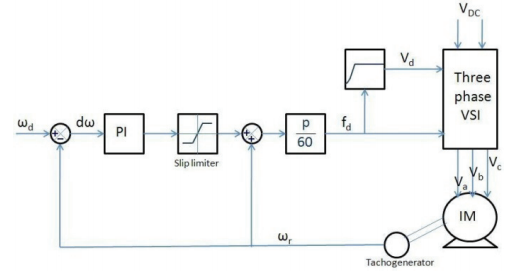
\includegraphics[width=1.0\linewidth]{vf_closed.png}
		\shorthandon{=}	
		\caption{V/f Tipik Kontrol Diyagramı}
		\label{fig:vf_kontrol}
	\end{figure}
	Şekil-\ref{fig:vf_kontrol} de ise skaler kontrol için genel blok diyagramı verilmiştir. Görüldüğü üzere yalnızca hız bilgisinin ölçülmesi makina kontrolü için yeterli olmaktadır.
	
	\section{Vektör Kontrol}
	Koordinat sistemi dönüşümü tabanlı matematiği bol ve fazla işlemci gücü gerektiren bir tekniktir. Uygulanabilirliği daha zordur. Alan akısını oluşturan akım ile tork akımı birbirlerinden bağımsız bir şekilde DC motorlarda olduğu gibi kontrol edilebilir. Dolayısıyla dinamik performansı skaler kontrole göre daha üstündür.
	
	\begin{figure}[hp]
		\centering	
		\shorthandoff{=}
		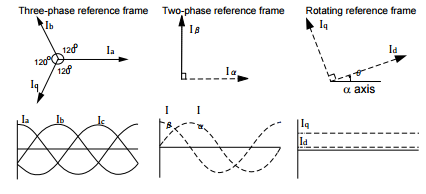
\includegraphics[width=0.7\linewidth]{clark_park.png}
		\shorthandon{=}	
		\caption{Vektör kontrol dönüşüm blokları}
		\label{fig:clark_park}
	\end{figure}
	
	Şekil-\ref{fig:clark_park}  vektör kontrolünün özünü oluşturan sırasıyla clark ve park dönüşümleri sonucunda elde edilen sinyaller görülmektedir. Clark dönüşümü sonucu, 3 faz aralarında  $120^\circ$ faz farkı bulunan 3 sinyal aralarında $90^\circ$ faz farkı bulunan 2 sinyale indirgenir.\newline
	Park dönüşümü sonucunda ise bu 2 adet sinyal eksen döndürme işleminin ardından DC bileşenlere dönüştürülür ve PI yada PID gibi kontrol teknikleri uygunalarak motor alan akısı ve tork bileşeni kolaylıkla kontrol edilebilir hale gelmiş olur.
	
	\begin{figure}[hp]
		\centering	
		\shorthandoff{=}
		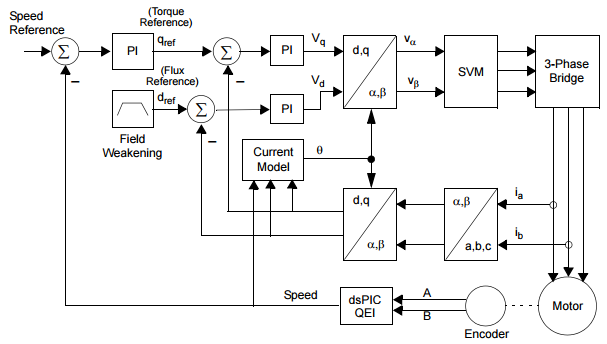
\includegraphics[width=0.7\linewidth]{foc_acim.png}
		\shorthandon{=}	
		\caption{Asenkron motorlar için FOC blok diyagramı}
		\label{fig:foc_acim}
	\end{figure}
	
	Şekil-\ref{fig:foc_acim} asenkron bir motor için FOC blok şeması verilmiştir. Asenkron motorlara özel olarak Current-Model bloğu içerisinde kayma değeri hesaplanır ve enkoder yada gözetleyiciden gelen pozisyon bilgisine dahil edilerek rotor akısının pozisyonu elde edilir. Motorun beklenen cevabı verebilmesi buradaki açının doğruluğuna bağlıdır.
	\newpage
	\section{Kıyaslama-Sonuç}
	Bahsedilen bu 2 yöntemin arasındaki öne çıkan en önemli fark ise akım, hız gibi bileşenlerin dinamik cevaplarıdır. Şekil-\ref{subfig:speed_scaler} ve şekil-\ref{subfig:speed_vector} hız için gösterilmiştir. 
	
	\begin{figure}[hp]
		\centering
		\begin{subfigure}[b]{0.4\textwidth}
			\shorthandoff{=}
			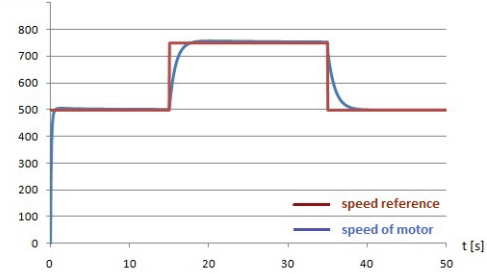
\includegraphics[width=\textwidth]{speed_scaler.png}
			\caption{Skaler}
			\label{subfig:speed_scaler}
			\shorthandon{=}
		\end{subfigure}
		~
		\begin{subfigure}[b]{0.4\textwidth}
			\shorthandoff{=}
			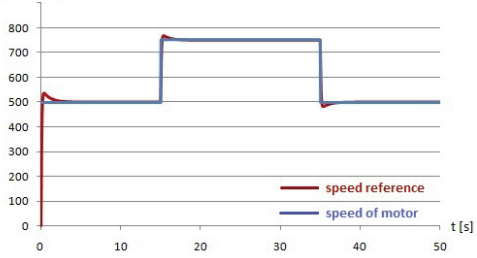
\includegraphics[width=\textwidth]{speed_vector.png}
			\caption{Vektörel}
			\label{subfig:speed_vector}
			\shorthandon{=}
		\end{subfigure}
	\end{figure}
	
	Skaler ve vektörel kontrol arasında öne çıkan farklar Tablo-\ref{tab:scaler_vector_tab} verildiği gibidir.
	
	\begin{center}
		\begin{table}[hb]
		\begin{tabular}{| l | c | c |}
			
			\hline
			 	 & Skaler Kontrol & Vektörel Kontrol \\ \hline
			 Maliyet & Ucuz & Pahalı  \\ \hline
			 Gerçeklenebilirlik & Kolay & Zor \\ \hline
			 Dinamik Karakteristik & Yavaş & Hızlı \\ \hline
			 Bağımsız Alan ve Tork Bileşeni Kontrolü & Yapılamaz & Yapılabilir \\ \hline
			 İşlem Gücü İhtiyacı & Az & Çok fazla \\ \hline
			 
			 
		\end{tabular}
		\caption{Skaler ve Vektöler Kontrol Kıyaslaması}
		\label{tab:scaler_vector_tab}
		\end{table}
	\end{center}
	
\end{document}